%%%%%%%%%%%%%%%
%
% $Autor:Abishek Senthilkumar $
% $Datum: 2022-06-16 06:54:43Z $
% $Pfad: WuSt/Skript/Produktspezifikation/powerpoint/NaiveBayesWithPython.tex $
% $Version: 4973 $
%
%
%%%%%%%%%%%%%%%




\Mysection{Introduction}

\STANDARD{What is Naive Bayes Classifier}
{
	Naive Bayes classifier  is a supervised-learning technique.
	
	\medskip
	
	We have samples of  data representative of different classes. Then using Bayes Theorem we calculate the probability of new data being in each class.
	
}

\begin{frame}{Why is it called Naïve Bayes?}
	
	\begin{itemize}
		\item \textbf{Naïve}: Assumes \textbf{feature independence}; each feature independently contributes to classification.
		\begin{itemize}
			\item Example: Identifies a fruit as an apple based on \textbf{color, shape}, and \textbf{taste}, assuming these features are independent.
			
			\begin{figure}
				\centering
				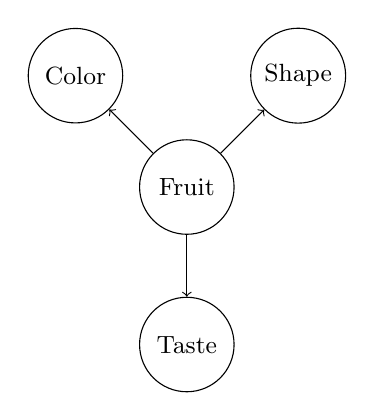
\begin{tikzpicture}[
					node distance=2.0cm,
					every node/.style={draw, circle, minimum size=1.2cm, text centered, font=\small}
					]
					% Nodes
					\node (class) {Fruit};
					\node[above left of=class] (color) {Color};
					\node[above right of=class] (shape) {Shape};
					\node[below of=class] (taste) {Taste};
					
					% Arrows representing independence
					\draw[->] (class) -- (color);
					\draw[->] (class) -- (shape);
					\draw[->] (class) -- (taste);
				\end{tikzpicture}
				\caption{Naïve Bayes Classifier Example}
				\label{fig:Naïve Bayes Classifier Example}
			\end{figure}
		\end{itemize}
	\end{itemize}
\end{frame}

\begin{itemize}
	\item \textbf{Bayes}: It is called Bayes because it depends on the principle of Bayes' Theorem.
	
	\medskip
	
	
	\textbf{Bayes' Theorem:} Also known as \textbf{Bayes' Rule} or \textbf{Bayes' Law}, it is used to determine the probability of a hypothesis based on prior knowledge and conditional probability.
	
	\bigskip
	The formula for Bayes' theorem is given by:
	\[
	P(A|B) = \frac{P(B|A) \cdot P(A)}{P(B)}
	\]
	
	\textbf{Where:}
	\begin{itemize}
		\item \( P(A|B) \): \textbf{Posterior Probability} - The probability of the hypothesis \( A \) given the observed event \( B \).
		\item \( P(B|A) \): \textbf{Likelihood Probability} - The probability of the evidence \( B \) given that hypothesis \( A \) is true.
		\item \( P(A) \): \textbf{Prior Probability} - The initial probability of the hypothesis \( A \) before observing any evidence.
		\item \( P(B) \): \textbf{Marginal Probability} - The probability of observing the evidence \( B \).
	\end{itemize}
\end{itemize}


\begin{frame}{When to use the Naïve Bayes Classifier algorithm:}
\begin{itemize}
	\item If you have a moderate or large training data set.
	\item If the instances have several attributes.
	\item Given the classification parameter, attributes which describe the instances should be conditionally independent.
\end{itemize}
\end{frame}

\begin{frame}{Applications of Naive Bayes Classifier}
	

	
	\begin{itemize}
		\item Sentiment Analysis: It is used at Facebook to analyse status updates expressing positive or negative emotions.
		\item Document Categorization: Google uses document classification to index documents and find relevancy scores i.e. the PageRank. PageRank mechanism considers the pages marked as important in the databases that were parsed and classified using a document classification technique.
		\item Naive Bayes Algorithm is also used for classifying news articles about Technology, Entertainment, Sports, Politics, etc.
		\item Email Spam Filtering-Google Mail uses Naive Bayes algorithm to classify your emails as Spam or Not Spam.
\end{itemize}
\end{frame}


\begin{frame}	{Types of Naïve Bayes Algorithms}
	
	
	
	Naïve Bayes has \textbf{3 main types}:
	\begin{itemize}
		\item \textbf{Gaussian Naïve Bayes}
		\item \textbf{Multinomial Naïve Bayes}
		\item \textbf{Bernoulli Naïve Bayes}
	\end{itemize}
\end{frame}

\begin{frame}{1. Gaussian Naïve Bayes}
	\textbf{Description}:
	\begin{itemize}
		\item Suitable for \textbf{continuous data}.
		\item Assumes data in each class follows a \textbf{Gaussian (Normal) distribution}.
		\item Requires calculation of \textbf{mean} (\(\mu\)) and \textbf{variance} (\(\sigma^2\)) for each class.
	\end{itemize}
	
	\textbf{Formula}:
	\[
	P(x | \text{Class}) = \frac{1}{\sqrt{2 \pi \sigma^2}} \exp \left( -\frac{(x - \mu)^2}{2 \sigma^2} \right)
	\]
	
	\textbf{Applications}:
	\begin{itemize}
		\item \textbf{Medical Diagnosis}: Predict diseases based on continuous indicators (e.g., blood pressure).
		\item \textbf{Iris Classification}: Classify flower species based on features like petal length.
	\end{itemize}
\end{frame}


\begin{frame}{2. Multinomial Naïve Bayes}
	\textbf{Description}:
	\begin{itemize}
		\item Designed for data that is \textbf{multinomially distributed} (e.g., frequency data).
		\item Suitable for \textbf{count-based data} such as word counts in text classification.
	\end{itemize}
	
	\textbf{Mechanism}:
	\begin{itemize}
		\item Treats feature vectors as \textbf{event frequencies} (e.g., word counts).
		\item Assumes each feature has a probability of occurrence.
	\end{itemize}
	
	\textbf{Applications}:
	\begin{itemize}
		\item \textbf{Text Classification}: Document categorization, spam detection, sentiment analysis.
		\item \textbf{Product Categorization}: Classify products based on descriptions by term frequencies.
	\end{itemize}
\end{frame}


\begin{frame}{3. Bernoulli Naïve Bayes}
	\textbf{Description}:
	\begin{itemize}
		\item Designed for \textbf{binary data} (0 or 1 values).
		\item Treats features as \textbf{boolean variables} representing presence or absence.
	\end{itemize}
	
	\textbf{Mechanism}:
	\begin{itemize}
		\item Considers whether a feature occurs (1) or does not occur (0).
	\end{itemize}
	
	\textbf{Applications}:
	\begin{itemize}
		\item \textbf{Document Classification}: Identify documents based on keyword presence (e.g., spam detection).
		\item \textbf{Image Recognition}: Classify binary images based on presence of specific features.
	\end{itemize}
\end{frame}







\Mysection{The problem}

\STANDARD{Naive Bayes}
{
	Think about targeted marketing:
	
	\begin{itemize}
		\item Users in specific age ranges with interest in certain products
		\item Users with specific income levels that indicate purchasing power
		\item  For-profit organizations using data to predict customer buying behavior
		\item \ldots
	\end{itemize}
	
	\bigskip
	
	$\Rightarrow\quad$ Need of a predictive model for user behavior
}  




\Mysection{Naive Bayes model using Python}


{
	
	
	% Slide 1: Dataset Introduction
	\begin{frame}{Dataset Introduction}
		\textbf{Objective:} Predict whether a user will make a purchase based on their age and salary.
		
		\textbf{Features:}
		\begin{itemize}
			\item \textbf{Age}: User’s age in years (numerical).
			\item \textbf{Salary}: User’s annual salary (numerical).
			\item \textbf{Purchase (Target Variable)}: 1 (purchase), 0 (no purchase).
		\end{itemize}
	\end{frame}
	
	% Slide 2: Example Data Entries
	\begin{frame}{Example Data Entries}
		\begin{tabular}{|c|c|c|}
			\hline
			\textbf{Age} & \textbf{Salary} & \textbf{Purchase} \\
			\hline
			22 & 45,000 & 0 \\
			34 & 60,000 & 1 \\
			45 & 80,000 & 1 \\
			29 & 50,000 & 0 \\
			52 & 120,000 & 1 \\
			\hline
		\end{tabular}
	\end{frame}
	
	% Slide 3: Objective
	\begin{frame}{Objective}
		\textbf{Goal:} Use age and salary data to predict whether a user will make a purchase.
		
		\textbf{Model:} Naïve Bayes classifier, assuming age and salary are independent in predicting the likelihood of a purchase.
	\end{frame}
	
}


% Slide 1: Naïve Bayes Formula
\begin{frame}{Naïve Bayes Formula}
	The Naïve Bayes model is based on Bayes’ theorem:
	\[
	P(B|X) = \frac{P(X|B) \cdot P(B)}{P(X)}
	\]
	\begin{itemize}
		\item \(P(B|X)\): Probability of purchase, given Age and Salary.
		\item \(P(X|B)\): Probability of observing Age and Salary, given that the user purchased the product.
		\item \(P(B)\): Prior probability of purchase.
		\item \(P(X)\): Probability of observing Age and Salary.
	\end{itemize}
\end{frame}

% Slide 2: Independence Assumption
\begin{frame}{Independence Assumption}
	Naïve Bayes assumes independence between Age and Salary:
	\[
	P(X|B) = P(\text{Age}|B) \times P(\text{Salary}|B)
	\]
\end{frame}

% Slide 3: Gaussian Naïve Bayes
\begin{frame}{Gaussian Naïve Bayes}
	For continuous features, Gaussian Naïve Bayes assumes a normal distribution:
	\[
	P(x|B) = \frac{1}{\sqrt{2\pi \sigma^2}} \exp \left( -\frac{(x - \mu)^2}{2 \sigma^2} \right)
	\]
	where:
	\begin{itemize}
		\item \(\mu\) is the mean.
		\item \(\sigma^2\) is the variance for each feature (Age or Salary).
	\end{itemize}
\end{frame}


\Mysection{Implementation}
\begin{frame}{Packages}

For building this model, we leverage several key Python libraries to handle data manipulation, analysis, model building, and evaluation for predicting purchase behavior.



\begin{itemize}
	\item \textbf{Pandas}
	\textbf{Purpose:} Powerful library for data manipulation and analysis.
	
	\textbf{Usage}
	\begin{itemize}
		\item Read, inspect, clean, and preprocess the dataset.
		\item Load data into DataFrame, handle missing values, filter, sort, and perform statistical analysis.
	\end{itemize}
	
	
	
	\item\textbf{NumPy}
	\textbf{Purpose:} Supports high-performance mathematical and statistical operations on large arrays.
	
	\textbf{Usage:}
	\begin{itemize}
		\item Perform numerical calculations for probability estimation.
		\item Handle feature transformations and vectorized calculations.
	\end{itemize}
\end{itemize}
\end{frame}

\begin{itemize}
	\item\textbf{Scikit-Learn (sklearn)}
	\textbf{Purpose:} Machine learning library for data preprocessing, model building, evaluation, and tuning.
	
	\textbf{Usage:}
	\begin{itemize}
		\item \textbf{Train-Test Split:} Split dataset into training/testing subsets.
		\item \textbf{Naïve Bayes Model:} Use GaussianNB for continuous features (age, salary).
		\item \textbf{Performance Metrics:} Evaluate using accuracy, precision, recall, and confusion matrix .
	\end{itemize}
	
	
	
	\item\textbf{Matplotlib and Seaborn}
	\textbf{Purpose:} Popular libraries for data visualization.
	
	\textbf{Usage:}
	\begin{itemize}
		\item \textbf{Matplotlib:} Create histograms and scatter plots for feature distributions.
		\item \textbf{Seaborn:} Create heatmaps and confusion matrix visualizations.
	\end{itemize}
\end{itemize}


\begin{itemize}
\item\textbf{ re (Regular Expressions)}
\textbf{Purpose:} Allows text manipulation and pattern extraction.
\textbf{Usage:}
\begin{itemize}
	\item Clean or standardize text-based features (e.g., categorical data).
	\item Extract patterns if the dataset has textual features.
\end{itemize}
\end{itemize}


\begin{python}
import numpy as np
import pandas as pd
from sklearn.model_selection import train_test_split
from sklearn.preprocessing import StandardScaler
from sklearn.naive_bayes import GaussianNB
from sklearn.metrics import confusion_matrix, accuracy_score
import matplotlib.pyplot as plt
from matplotlib.colors import ListedColormap
\end{python}


\STANDARD{Data Pre-Processing}

We load the dataset from a CSV file:
\begin{itemize}
	\item \texttt{X}: Contains the features (Age and Estimated Salary).
	\item \texttt{y}: Target variable (Purchased).
\end{itemize}
\begin{python}
	import pandas as pd
	
	# Load dataset
	dataset = pd.read_csv('SocialNetworkAds.csv')
	
	# Extract features (Age and Estimated Salary) and target (Purchased)
	X = dataset.iloc[:, [2, 3]].values  # Features
	y = dataset.iloc[:, -1].values  # Target
\end{python}



	
	Next, we split the data into training and testing sets:
	
	\begin{itemize}
	\item 75\% for training and 25\% for testing.
	\item traintestsplit() ensures random splitting, allowing for unbiased evaluation.
    \end{itemize}

	\begin{python}
X_train, X_test, y_train, y_test = train_test_split(X, y, test_size=0.25, random_state=0)
\end{python}
	This ensures that 75\% of the data is used for training and 25\% for testing. The \texttt{train\_test\_split()} function randomly splits the data, allowing for unbiased evaluation.
	

Since the features (Age and Estimated Salary) may have different scales, we scale them to ensure that the model performs optimally. We apply standard scaling to both training and testing data.
	\begin{python}
		sc = StandardScaler()
		X_train = sc.fit_transform(X_train)
		X_test = sc.transform(X_test)
		
\end{python}


\STANDARD{Training the Naive Bayes Model}

 We initialize a Gaussian Naive Bayes classifier and train it using the scaled training data \texttt{(Xtrain and ytrain)}.
 	\begin{python}
classifier = GaussianNB()
classifier.fit(X_train, y_train)
\end{python}
\STANDARD{Prediction and Evaluation}

We use the predict function to make predictions on the test set .
\begin{python}
y_pred = classifier.predict(X_test)
\end{python}
To evaluate the performance of the model, we:
\begin{itemize}
\item Use a confusion matrix to analyze the true positives, false positives, true negatives, and false negatives.
\item Calculate the accuracy score, which indicates how well the model performs.
\end{itemize}
\begin{python}
cm = confusion_matrix(y_test, y_pred)
accuracy = accuracy_score(y_test, y_pred)
print("Confusion Matrix:\n", cm)
print("Accuracy:", accuracy)
\end{python}



	
\STANDARD{Visualizing the Training Set Results}

To better understand the model's predictions, we visualize the decision boundary and the data points in the training set. The contourf function helps create a decision boundary, and the scatter function plots the actual data points.
\begin{python}
X_set, y_set = X_train, y_train
X1, X2 = np.meshgrid(np.arange(start=X_set[:, 0].min() - 1, stop=X_set[:, 0].max() + 1, step=0.01),
np.arange(start=X_set[:, 1].min() - 1, stop=X_set[:, 1].max() + 1, step=0.01))
plt.contourf(X1, X2, classifier.predict(np.array([X1.ravel(), X2.ravel()]).T).reshape(X1.shape),
alpha=0.75, cmap=ListedColormap(('red', 'green')))
plt.xlim(X1.min(), X1.max())
plt.ylim(X2.min(), X2.max())
for i, j in enumerate(np.unique(y_set)):
plt.scatter(X_set[y_set == j, 0], X_set[y_set == j, 1],
c=ListedColormap(('red', 'green'))(i), label=j)
plt.title('Naive Bayes (Training set)')
plt.xlabel('Age')
plt.ylabel('Estimated Salary')
plt.legend()
plt.show()
\end{python}

\begin{figure}[h!]
	\centering
	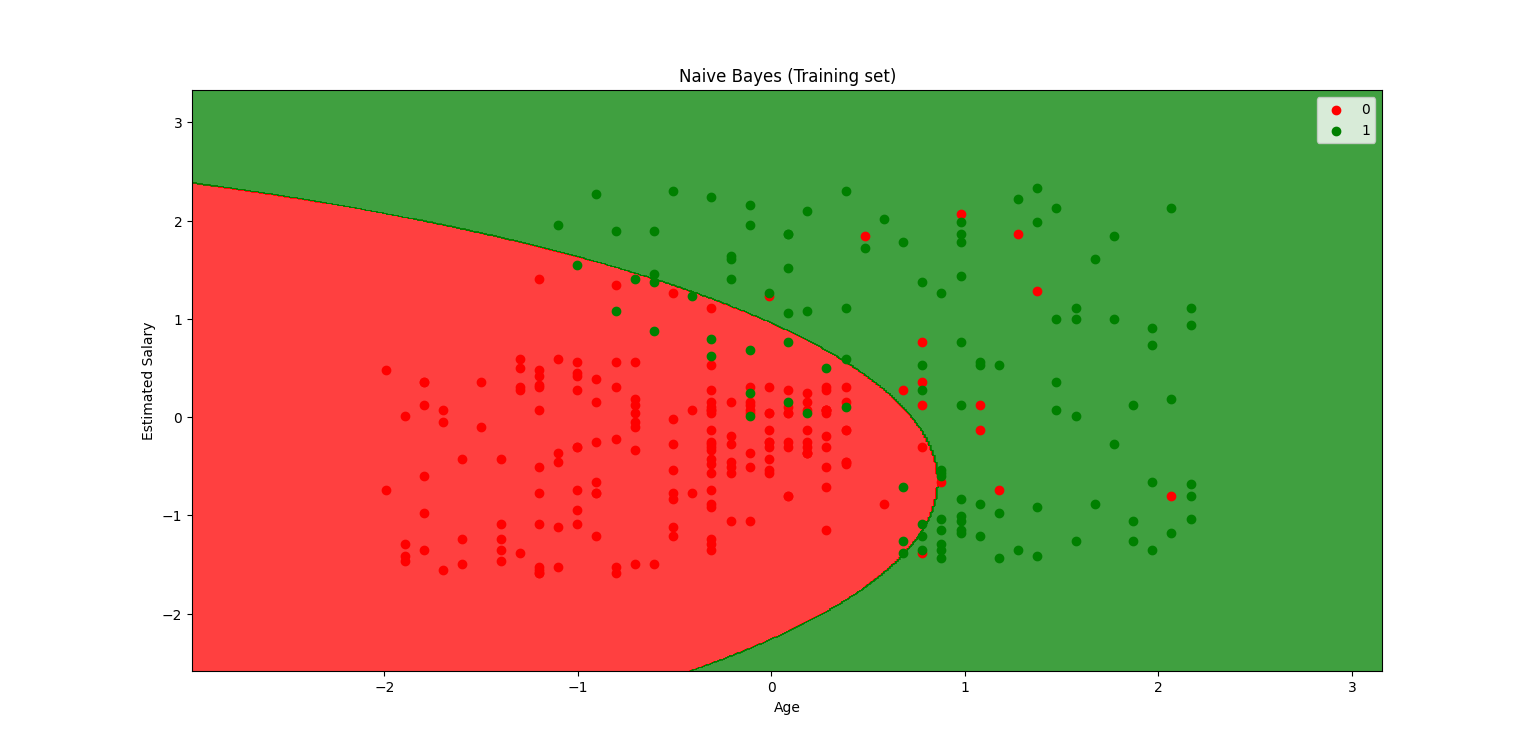
\includegraphics[width=1\textwidth, height=5cm]{Images/NaiveBayestrainset.png}
	\caption{Training set}
	\label{Output Train}
\end{figure}
\STANDARD{Visualizing the Test Set Results}
The same visualization approach is used to plot the decision boundary and data points for the test set.
\begin{python}
X_set, y_set = X_test, y_test
X1, X2 = np.meshgrid(np.arange(start=X_set[:, 0].min() - 1, stop=X_set[:, 0].max() + 1, step=0.01),
np.arange(start=X_set[:, 1].min() - 1, stop=X_set[:, 1].max() + 1, step=0.01))
plt.contourf(X1, X2, classifier.predict(np.array([X1.ravel(), X2.ravel()]).T).reshape(X1.shape),
alpha=0.75, cmap=ListedColormap(('red', 'green')))
plt.xlim(X1.min(), X1.max())
plt.ylim(X2.min(), X2.max())
for i, j in enumerate(np.unique(y_set)):
plt.scatter(X_set[y_set == j, 0], X_set[y_set == j, 1],
c=ListedColormap(('red', 'green'))(i), label=j)
plt.title('Naive Bayes (Test set)')
plt.xlabel('Age')
plt.ylabel('Estimated Salary')
plt.legend()
plt.show()
\end{python}
\begin{figure}[h!]
	\centering
	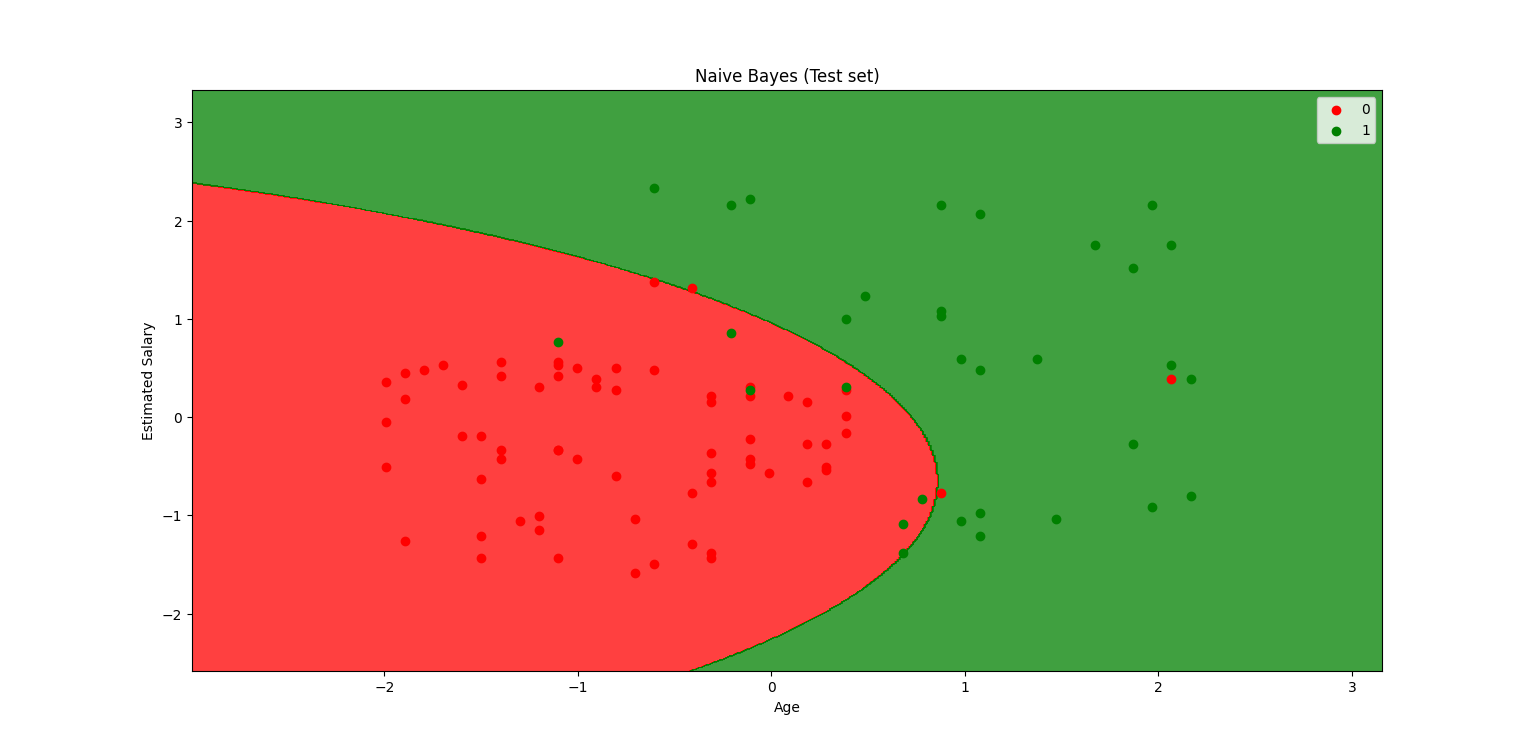
\includegraphics[width=1\textwidth, height=5cm]{Images/NaiveBayestestset.png}
	\caption{Test set}
	\label{Output Test}
\end{figure}


	

	
	\begin{frame}{Naive Bayes Hyperparameters}
		\begin{itemize}
		
			
			\item \textbf{Key Hyperparameters for Fine-Tuning}
			\begin{itemize}
				\item \textbf{var\_smoothing}: Controls smoothing applied to the variance to prevent instability.
				\item \textbf{priors}: Sets prior probabilities for each class; useful for known or imbalanced class distributions.
				\item \textbf{fit\_prior}: Boolean flag to determine if priors are learned from the data or set manually.
			\end{itemize}
		\end{itemize}
	\end{frame}
	
\begin{frame}{Understanding the Impact of Each Hyperparameter}
	\begin{itemize}
		\item \textbf{1. Variance Smoothing (\texttt{var-smoothing})}
		\begin{itemize}
			\item \textbf{Purpose}: Adds a small constant to feature variance to avoid division by zero.
			\item \textbf{Effect}: 
			\begin{itemize}
				\item Higher values: More generalized model (better for noisy data).
				\item Lower values: Potential overfitting due to sensitivity to small variance differences.
			\end{itemize}
		
		\end{itemize}
		
		\item \textbf{2. Class Prior Probabilities (\texttt{priors})}
		\begin{itemize}
			\item \textbf{Purpose}: Allows specifying likelihood of each class.
			\item \textbf{Effect}: Useful for imbalanced datasets (e.g., more users who don’t purchase).
		
		\end{itemize}
			\end{itemize}
			\end{frame}
		\begin{itemize}	
		\item \textbf{3. Fit Priors (\texttt{fit-prior})}
		\begin{itemize}
			\item \textbf{Purpose}: Controls if priors are computed from data (\texttt{True}) or set manually.
			\item \textbf{Effect}:
			\begin{itemize}
				\item \texttt{True}: Model learns class priors from data.
				\item \texttt{False}: Requires manual setting of \texttt{priors}.
			\end{itemize}
		
		\end{itemize}
	\end{itemize}

\begin{python}
	classifier = GaussianNB(var-smoothing=1e-7)
	classifier = GaussianNB(fit-prior=False)
	classifier = GaussianNB(priors=[0.7, 0.3])
		\end{python}
		\Mysection{Advantages of the Naive Bayes Classifier}
		\STANDARD{Advantages of the Naive Bayes Classifier Algorithm}
		{
			\begin{enumerate}
				\item Naive Bayes Classifier algorithm performs well when the input variables are categorical
				\item A Naive Bayes classifier converges faster, requiring relatively little training data than other discriminative models like logistic regression, when the Naive Bayes conditional independence assumption holds.
				\item With Naive Bayes Classifier algorithm, it is easier to predict class of the test data set. A good bet for multi class predictions as well.
				\item 	Though it requires conditional independence assumption, Naive Bayes Classifier has presented good performance in various application domains.
			\end{enumerate}
		}	
		\Mysection{Limitations and Improvements}
	\begin{frame}
		\frametitle{Limitations of Naive Bayes}
		
		\begin{itemize}
			\item \textbf{Assumption of Feature Independence:} \\
			Naive Bayes assumes that features are conditionally independent, which is often unrealistic and can lead to oversimplified models.
			
			\item \textbf{Sensitivity to Irrelevant Features:} \\
			Irrelevant or redundant features can negatively impact performance, as Naive Bayes doesn't automatically downweight less important features.
			
			\item \textbf{Handling Imbalanced Data:} \\
			Naive Bayes may struggle with imbalanced datasets, often becoming biased toward the majority class.
			
			\item \textbf{Limited Handling of Continuous Features:} \\
			Gaussian Naive Bayes assumes continuous features follow a normal distribution, which may not suit all datasets well.
			
			\item \textbf{Limited Model Flexibility:} \\
			The simplicity of Naive Bayes limits its ability to model complex relationships, making it unsuitable for some non-linear problems.
		\end{itemize}
	\end{frame}
	

	\begin{frame}
		\frametitle{Improvements for Naive Bayes}
		
		\begin{itemize}
			\item \textbf{Feature Engineering and Selection:} \\
			Use techniques like TF-IDF, n-grams, and mutual information to select and engineer impactful features.
			
			\item \textbf{Advanced Smoothing Techniques:} \\
			Apply alternative smoothing (e.g., Lidstone or Good-Turing) and optimize smoothing parameters to improve accuracy.
			
			\item \textbf{Techniques for Imbalanced Data:} \\
			Adjust class priors, apply cost-sensitive Naive Bayes, or use SMOTE to balance the dataset.
			
			\item \textbf{Hybrid and Ensemble Approaches:} \\
			Combine with algorithms (e.g., SVM) or use ensemble methods like AdaBoost for better generalization and accuracy.
			
			\item \textbf{Improved Handling of Continuous Features:} \\
			Use kernel density estimation for non-Gaussian distributions or discretize continuous variables for simpler modeling.
		\end{itemize}
		
	\end{frame}
	




